% perk
\begin{frame}{Signal Model}
	\uncover<+->{%
		\textbf{Given}: at every voxel, measurement vector $\bmy \in \complexes{D}$ modeled as 
		\begin{align}
			\bmy = \bms\paren{\bmx,\bmnu} + \bmeps
			\label{eq:model}
		\end{align}
		\begin{itemize}
			\item{\makebox[3cm][l]{$\bmx \in \reals{L}$} unknown parameters}
			\item{\makebox[3cm][l]{$\bmnu \in \reals{K}$} ``known'' parameters}
			\item{\makebox[3cm][l]{$\bms : \reals{L+K} \mapsto \complexes{D}$} 
				vector signal model}
			\item{%
				\makebox[3cm][l]{$\bmeps \in \complexes{D}$} 
				noise $\sim \cgauss{\zeros{D}}{\bmSig}$
			}%
		\end{itemize}
		\vspace{0.5cm}
	}%
	\uncover<+->{%
		\textbf{Task}: design fast voxel-by-voxel estimator $\esta{\bmx}{\bmy,\bmnu}$
	}%
\end{frame}

\begin{frame}{Prior Work}
	\uncover<1->{%
		\textbf{Task}: design fast voxel-by-voxel estimator $\esta{\bmx}{\bmy,\bmnu}$
  	
  	\textbf{Challenges}:
  	\begin{itemize}
  		\item{signal $\bms$ often nonlinear in $\bmx$: non-convex inverse problems}
  		\item{signal $\bms$ might be difficult to write in closed form}
  	\end{itemize}
	}%
	\uncover<2->{%
  	\textbf{Conventional Approaches:}
	}%
  	\begin{itemize}
			\item<2-3>{gradient-based local optimization}
			\begin{itemize}
				\item{initialization-dependent solution}
				\item{requires signal gradients}
			\end{itemize}
  		\item<3>{stochastic methods (\eg, simulated annealing)}
  		\begin{itemize}
  			\item{unclear convergence analysis \hfill \citec{bertsimas:93:sa}}
  			\item{several unintuitive tuning parameters}
  		\end{itemize}
			\item<4>{%
				dictionary-based grid search
			}%
  	\end{itemize}
\end{frame}

\begin{frame}{Motivation}
	\textbf{Grid search} computational costs
	\begin{table}
		\centering
		\begin{tabular}{r|cc}
			& $L$ & $\sim$number dictionary atoms \\
			\hline
			\uncover<1-2>{1-compartment relaxivity 		& 3 		& $\sim$$100^2$ \\}
			\uncover<2>{flow velocity 									& 4 		& $\sim$$100^3$ \\} 
			\uncover<2>{diffusivity tensor 							& 7 		& $\sim$$100^6$ \\}
			\uncover<2->{\hlg{2-3 compartment relaxivity}& 6-10 	& $\sim$$100^5-100^9$} 
			\end{tabular}
		\end{table}
		
		\uncover<3>{
			\textbf{Can we scale computation with $L$ more gracefully?}
		}
\end{frame}

\begin{frame}{Machine Learning for QMRI Parameter Estimation}
	\uncover<1->{%
		\textbf{Idea}: learn a \emph{nonlinear} estimator from simulated training data
	}
	\begin{itemize}
		\item<2-3>{%
			sample $\paren{\bmx_1,\bmnu_1,\bmeps_1},\dots,\paren{\bmx_N,\bmnu_N,\bmeps_N}$
			from prior distributions
		}
		\item<2-3>{%
			simulate image data vectors $\bmy_1,\dots,\bmy_N$ 
			via signal model $\bms$
		}
		\item<3-5>{%
			design \emph{nonlinear} functions 
				$\est{x}_l\paren{\cdot} := \est{h}_l\paren{\cdot} + \est{b}_l$ 
				for $l \in \set{1,\dots,L}$ \\
				that map each 
				$\bmq_n := [\re{\bmy_n}\tpose, \im{\bmy_n}\tpose, \bmnu_n\tpose]\tpose \in \setQ$	
				to $x_{l,n} \in \real$
		}
	\end{itemize}	
	\vspace{-0.3cm}
	\uncover<4->{%
		\alt<4-5>{%
			\begin{align}
				\paren{\est{h}_l,\est{b}_l} \in \set{
					\argmin{\substack{h_l \\ b_l \in \real}} 
					\frac{1}{N} \sum_{n=1}^N \paren{h_l\paren{\bmq_n} + b_l - x_{l,n}}^2
				}%
				\uncover<5>{%
					\,\,\,\,\, \textcolor{red}{\text{ill-posed!}}
				}%
				\nonumber
			\end{align}
		}{%
			\begin{align}
				\paren{\est{h}_l,\est{b}_l} \in \set{%
					\argmin{\substack{h_l \hlb{\in \hilb} \\ b_l \in \real}}
					\frac{1}{N} \sum_{n=1}^N \paren{h_l\paren{\bmq_n} + b_l - x_{l,n}}^2
					\hlb{+ \rho_l \norm{h_l}^2_\hilb}
				}%
				\label{eq:krr,cost}
			\end{align}
		}%
	}%
	\uncover<6->{%
		\textbf{Solution}: Param Estimation via Regression with \hlm{Kernels} (PERK) \\
			\hfill \citec{nataraj::dfm}%
		\begin{itemize}
			\item{restrict optimization to a \hlb{certain rich function space $\hilb$}}
			\item{optimal $\est{h}_l \hlb{\in \hilb}$ takes form 
				$\est{h}_l = \sum_{n=1}^N \est{a}_{l,n} \hlm{k}(\cdot,\bmq_n)$ \\
				\hfill \citec{scholkopf:01:agr}}
		\end{itemize}
	}	
\end{frame}

\begin{frame}{PERK in a 1-D Toy Problem}
	\uncover<1->{%
		\textbf{Task}: 
			estimate $\Tt$, given samples from $y = \exp\paren{-\TE/\Tt} + \epsilon$
		\vspace{-0.5cm}
		\begin{figure}
			\subfloat[$N\gets10$]{%
				\includegraphics [width=0.33\textwidth] {%
					c,perk/toy/toy-1d,t2-se,n-10%
				}%
			}%
			\subfloat[$N\gets20$]{%
				\includegraphics [width=0.33\textwidth] {%
					c,perk/toy/toy-1d,t2-se,n-20%
				}%
			}%
			\subfloat[$N\gets50$]{%
				\includegraphics [width=0.33\textwidth] {%
					c,perk/toy/toy-1d,t2-se,n-50%
				}%
			}%
		\end{figure}
	}%
	\uncover<1->{%
		\textbf{Compare}: $\TtPERK$ with method-of-moments (MOM) estimator 
			$$\TtMOM\paren{\cdot} := -\TE/\log{\abs{\cdot}}$$
		(PERK more useful when good MOM estimator unavailable)
	}%
\end{frame}

\begin{frame}{PERK Solution}
	Non-iterative closed-form solution, for $l \in \set{1,\dots,L}$: 
	\begin{align}
		\est{x}_l\paren{\cdot} = \bmxg{l}\tpose\paren{
			\frac{1}{N}\ones{N} 
			+ \bmM\inv{\bmK\bmM + N\rho_l \eye{N}} 
			\paren{\bmka{\cdot} - \frac{1}{N}\bmK\ones{N}}
		}
		\label{eq:krr,x-hat}
	\end{align}
	\begin{itemize}
	\item<1-4>{%
		\makebox[6cm][l]{$\bmxg{l} := [x_{l,1},\dots,x_{l,N}]\tpose$}
		training pt regressands
	}
	\item<2-4,6>{%
		\makebox[6cm][l]{%
			$\bmK := 
				\begin{bmatrix}
					\hlm{k}(\bmq_1,\bmq_1) 	& \cdots 	& \hlm{k}(\bmq_1,\bmq_N) \\
					\vdots									& \ddots	& \vdots \\
					\hlm{k}(\bmq_N,\bmq_1) 	& \cdots 	& \hlm{k}(\bmq_N,\bmq_N)
				\end{bmatrix}$
		}
		Gram matrix
	}						
	\item<3-4>{%
		\makebox[6cm][l]{$\bmM := \eye{N} - \frac{1}{N}\ones{N}\ones{N}\tpose$}
		de-meaning operator
	}
	\item<4>{%
		\makebox[6cm][l]{%
			$\bmka{\cdot} := \brac{\hlm{k}(\cdot,\bmq_1),\dots,\hlm{k}(\cdot,\bmq_N)}\tpose$
		}
		nonlin kernel embedding
	}
	\end{itemize}
	\uncover<5>{%
		Can we scale computation with $L$ more gracefully?
	}
	\begin{itemize}
		\item<5>{Perhaps, since \eqref{eq:krr,x-hat} separable in $l \in \set{1,\dots,L}$ by construction}
		\item<6>{However, explicitly computing $\bmK$ may be undesirable...}
	\end{itemize}
\end{frame}

\begin{frame}{PERK as High-Dimensional Affine Regression}
	\uncover<1->{
		Suppose there exists``approximate feature mapping'' $\bmztZ : \setQ \mapsto \reals{Z}$ \\
		such that $\bmZt := \brac{\bmztZa{\bmq_1},\dots,\bmztZa{\bmq_N}}$ has for $\dim\paren{\setQ} \ll Z \ll N$
		\begin{align}
			\bmK \approx \bmZt\tpose \bmZt.
			\label{eq:low-rank}
		\end{align}
		\vspace{-0.5cm}
	}
	\uncover<2-3>{%
		\begin{overlayarea}{\textwidth}{2.5cm}
  		\alt<2>{%
    		Plugging \eqref{eq:low-rank} into PERK solution \eqref{eq:krr,x-hat} and rearranging gives
    		\begin{align}
    			\est{x}_l\paren{\cdot} \approx 
    				\frac{1}{N}\bmxg{l}\tpose\ones{N} 
    				+ \frac{1}{N}\bmxg{l}\tpose \bmM \bmZt\tpose
    				\inv{\frac{1}{N} \bmZt \bmM \bmZt\tpose + \rho_l\eye{Z}}
    				\paren{\bmztZa{\cdot}-\frac{1}{N}\bmZt\ones{N}}
    				\nonumber
    		\end{align}
    	}{%
    		Plugging \eqref{eq:low-rank} into PERK solution \eqref{eq:krr,x-hat} and rearranging gives
    		\begin{align}
    			\est{x}_l\paren{\cdot} \approx 
    				\mxl + \cxlzt \inv{\Cztzt + \rho_l\eye{Z}} \paren{\bmztZa{\cdot} - \bmmzt}
    				\label{eq:x-cme}
    		\end{align}
				which is regularized $Z$-dimensional affine regression!
    	}
		\end{overlayarea}
	}
	\uncover<4->{%
		Does such a $\bmzt$ exist and work well in practice?
		\begin{itemize}
			\item{Yes, \eg for Gaussian
				$\hlm{k}(\bmq,\bmq') \gets \expa{-\frac{1}{2}\norm{\bmL^{-1}\paren{\bmq-\bmq'}}_2^2}$ \\
				\hfill \citec{rahimi:07:rff}}
			\item{In such cases, can reduce from $\sim$$N^2$ to $\sim$$NZ$ computations}
		\end{itemize}
	}
\end{frame}

\begin{frame}{Experimental Setup}
	\uncover<1->{%
		Demonstrated PERK for $\To,\Tt$ est from optim (2SP,1DE) scan
	}%
	\begin{itemize}
		\item<2>{%
			PERK trained using $N \gets 10^5$ samples from prior dist $\dist{\bmx,\bmnu}$
		}%
		\item<2>{%
			To enable precise estimation,
			support of $\dist{\bmx,\bmnu}$ carefully chosen \\
			to coincide with min-max acquisition design support
		}%
	\end{itemize}
	
	\uncover<3->{%
		Compared PERK to two well-suited ML estimators:
		\begin{itemize}
			\item{%
				dictionary-based grid search estimator via \\
				variable projection method (VPM) \hfill \citec{golub:03:snl}
			}%
			\item{%
				local optim estimator via preconditioned variant (PGPM) \\
				of classical gradient projection method \hfill \citec{rosen:60:tgp}
			}%
		\end{itemize}
	}%
\end{frame}
	
\begin{frame}{Phantom Results}
	\vspace{-0.3cm}
	\uncover<1->{%
  	\begin{figure}
			\centering
			\begin{minipage}{0.7\textwidth}
  			\subfloat{%
  				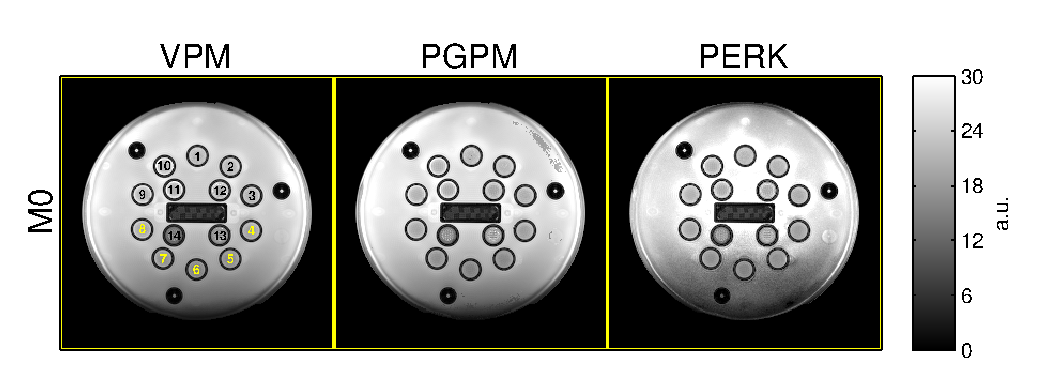
\includegraphics [width=0.96\textwidth,clip] {%
  					c,perk/hpd-tight/sp2de1,sl-6,m0,im-gray.eps%
  				}%
  			}%
  			\hspace{0cm}
    		\subfloat{%
  				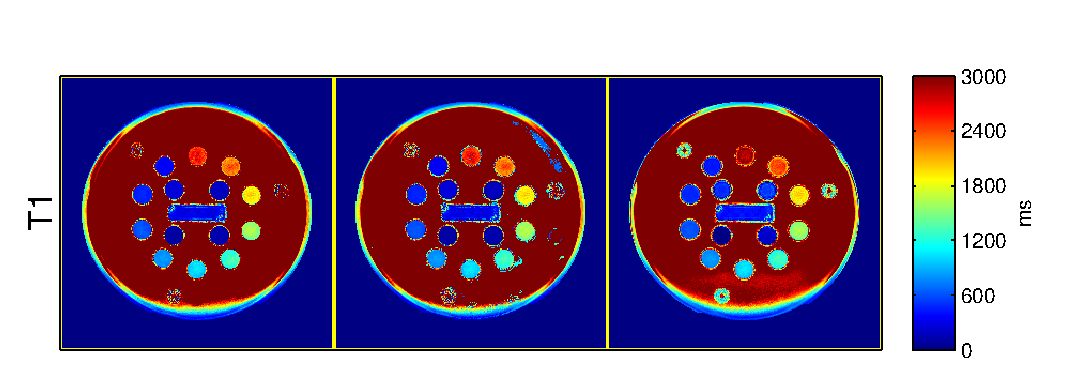
\includegraphics [width=0.982\textwidth,trim=0 0 0 25,clip] {%
  					c,perk/hpd-tight/sp2de1,sl-6,t1,im-jet.eps%
  				}%
  			}%
  			\hspace{0cm}
    		\subfloat{%
  				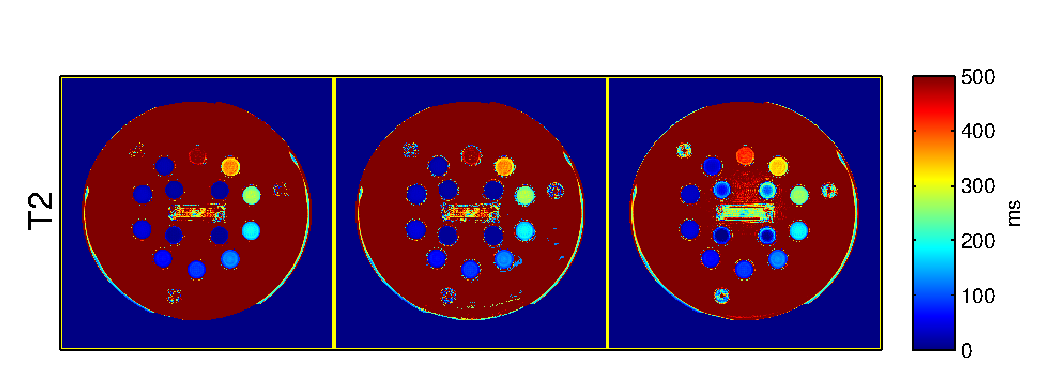
\includegraphics [width=0.97\textwidth,trim=0 0 0 25,clip] {%
  					c,perk/hpd-tight/sp2de1,sl-6,t2,im-jet.eps%
  				}%
  			}%
			\end{minipage}
			\label{fig:perk,hpd-tight,im}
  	\end{figure}
	}%
	\vspace{-0.3cm}
	\uncover<2->{%
		\makebox[3.3cm][r]{$928$s}
		\makebox[1.9cm][r]{$1257$s}
		\makebox[2.1cm][r]{$4.2$s train} \\
		\vspace{-0.1cm}
		\makebox[7.4cm][r]{$1.9$s test}
	}	
\end{frame}
	
\begin{frame}{Phantom Results}
	\uncover<1->{%
  	\begin{figure}
  		\centering
  		\subfloat{%
				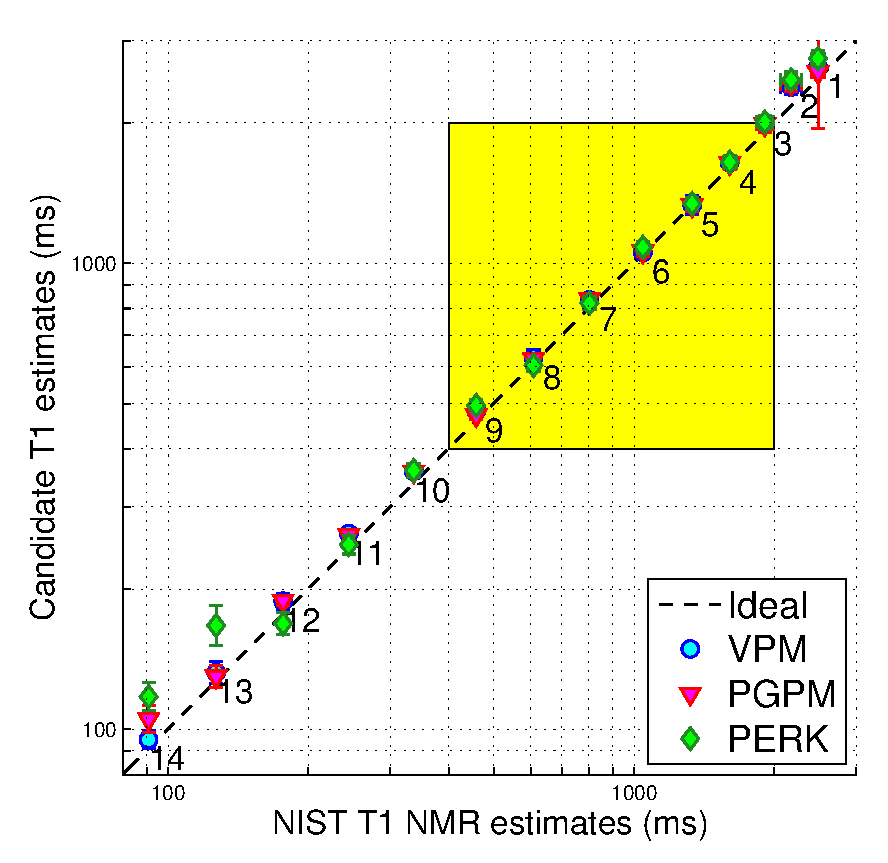
\includegraphics [width=0.45\textwidth] 
          {c,perk/hpd-tight/sp2de1,sl-6,t1,plot.eps}
        \label{fig:perk,hpd,plot,t1}
      }%
      \hspace{0.3cm}
      \subfloat{%
      	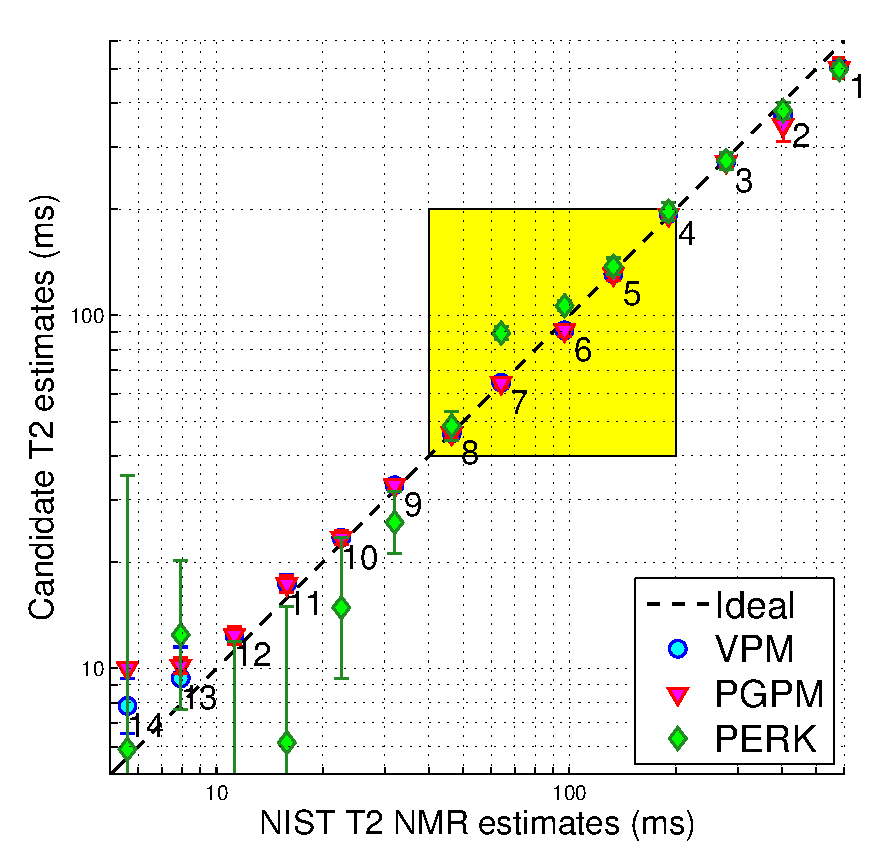
\includegraphics [width=0.45\textwidth] 
					{c,perk/hpd-tight/sp2de1,sl-6,t2,plot.eps}
				\label{fig:perk,hpd,plot,t2}
      }%
      \label{fig:perk,hpd-tight,plot}
   	\end{figure}
	}%
	\uncover<2->{%
		Within support of $\dist{\bmx,\bmnu}$, \\
		\textbf{PERK and grid search estimates agree excellently}.
	}%
\end{frame}

\begin{frame}{\emph{In vivo} Results}
	\vspace{-0.3cm}
	\uncover<1->{%
  	\begin{figure}
			\centering
			\begin{minipage}{0.6\textwidth}
  			\subfloat{%
  				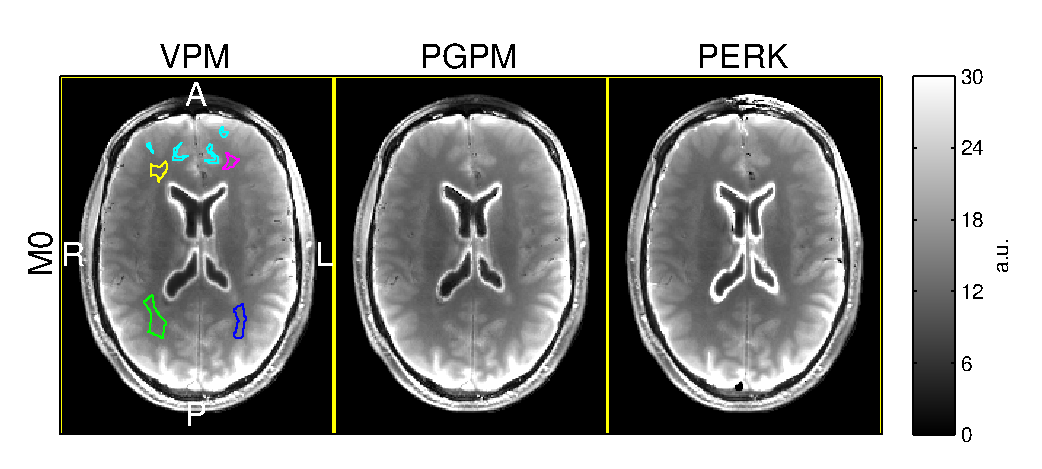
\includegraphics [width=0.96\textwidth,trim=0 0 0 10,clip] {%
  					c,perk/brain/sp2de1,sl-5,m0,im-gray.eps%
  				}%
  			}%
  			\hspace{0cm}
    		\subfloat{%
  				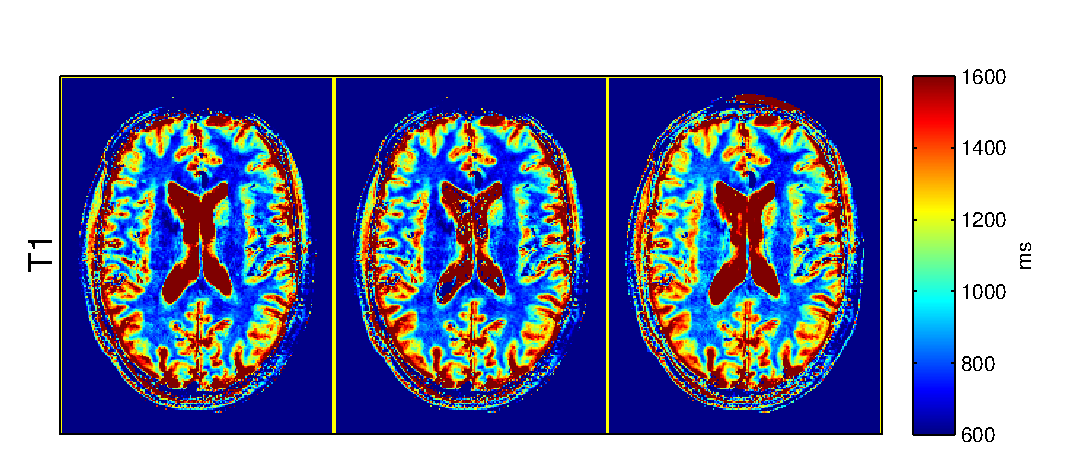
\includegraphics [width=0.982\textwidth,trim=0 0 0 20,clip] {%
  					c,perk/brain/sp2de1,sl-5,t1,im-jet.eps%
  				}%
  			}%
  			\hspace{0cm}
    		\subfloat{%
  				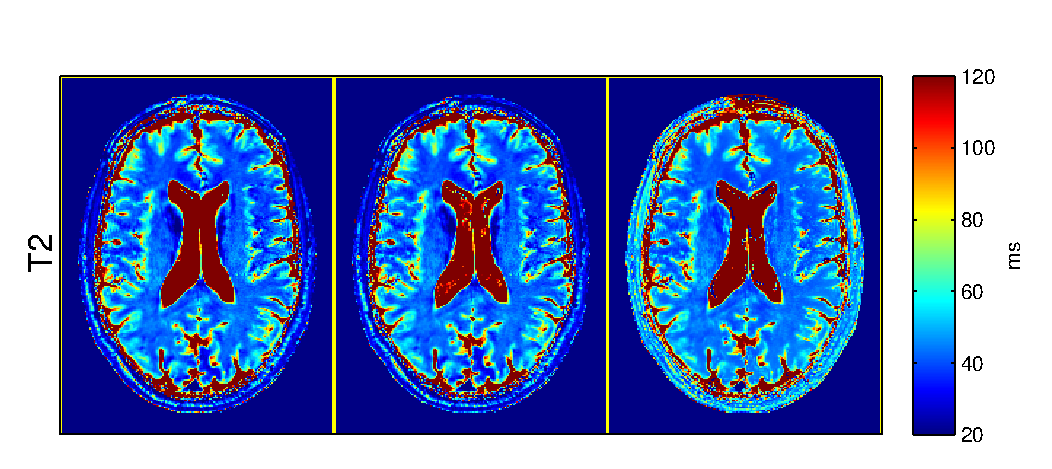
\includegraphics [width=0.97\textwidth,trim=0 0 0 20,clip] {%
  					c,perk/brain/sp2de1,sl-5,t2,im-jet.eps%
  				}%
  			}%
			\end{minipage}
			\label{fig:perk,hpd-tight}
  	\end{figure}
	}%
	\vspace{-0.3cm}
	\uncover<2->{%
		\makebox[3.6cm][r]{$838$s}
		\makebox[1.65cm][r]{$2178$s}
		\makebox[1.9cm][r]{$4.2$s train} \\
		\vspace{-0.1cm}
		\makebox[7.3cm][r]{$1.6$s test}
	}
\end{frame}

\begin{frame}{Summary}
	\uncover<1->{%
		\textbf{Contributions}
		\begin{itemize}
			\item<1->{\textbf{PERK}: fast, dictionary-free estimator for QMRI}
			\item<2->{demonstrated PERK for $\To,\Tt$ estimation}
			\begin{itemize}
				\item<2>{%
					Phantom (and omitted simulation) results show that \\
					PERK and ML estimators yield comparable accuracy/precision
				}
				\item<2>{%
					\emph{In vivo} PERK and ML estimates are comparable in WM/GM
				}
				\item<2-3>{%
					\textbf{PERK is consistently at least $140$x faster}
				}
			\end{itemize}
		\end{itemize}
	}
	\uncover<3>{%
		\textbf{Can we exploit PERK's speed in a more compelling problem?}
	}
\end{frame}
